\documentclass[aspectratio=169,11pt]{beamer}

% Theme
\usetheme{Madrid}
\usecolortheme{whale}
\useinnertheme{rectangles}

% Colors
\definecolor{darkblue}{HTML}{1B3A5C}
\definecolor{accentred}{HTML}{C0392B}
\definecolor{lightblue}{HTML}{3498DB}
\definecolor{darkgray}{HTML}{2C3E50}

\setbeamercolor{title}{fg=white,bg=darkblue}
\setbeamercolor{frametitle}{fg=white,bg=darkblue}
\setbeamercolor{structure}{fg=darkblue}
\setbeamercolor{block title}{fg=white,bg=darkblue}
\setbeamercolor{block body}{bg=darkblue!5}
\setbeamercolor{item}{fg=accentred}

% Packages
\usepackage[utf8]{inputenc}
\usepackage[T1]{fontenc}
\usepackage{lmodern}
\usepackage{booktabs}
\usepackage{graphicx}
\usepackage{tikz}
\usepackage{pgfplots}
\pgfplotsset{compat=1.18}

% Remove navigation
\setbeamertemplate{navigation symbols}{}
\setbeamertemplate{footline}[frame number]

% Title
\title[Indonesia Data Centers]{Data Centers in Indonesia}
\subtitle{Market Landscape, Investments, and Fiscal Cost of Tax Incentives}
\author{Working Paper}
\date{March 2026}

\begin{document}

% ============================================================
% SLIDE 1: Title + Market Overview
% ============================================================
\begin{frame}
\titlepage
\end{frame}

% ============================================================
% SLIDE 2: Market Snapshot & Key Players
% ============================================================
\begin{frame}{Indonesia Data Center Market at a Glance}

\begin{columns}[T]
\begin{column}{0.48\textwidth}
\begin{block}{Market Snapshot (2025)}
\begin{itemize}
    \item \textbf{88} existing facilities, \textbf{25} upcoming
    \item \textbf{307~MW} operational capacity
    \item Market value: \textbf{USD 2.81B} (2025)
    \item Projected: \textbf{USD 6.08B} by 2031
    \item IT load target: \textbf{3,560~MW} by 2030
\end{itemize}
\end{block}

\begin{block}{Geographic Split}
\begin{itemize}
    \item Jakarta: 56.7\% market share
    \item Batam: fastest growth (21.7\% CAGR)
    \item Pipeline: $\sim$670~MW across both hubs
\end{itemize}
\end{block}
\end{column}

\begin{column}{0.48\textwidth}
\begin{block}{Top Operators by Capacity (MW)}
\small
\begin{tabular}{lr}
\toprule
\textbf{Operator} & \textbf{MW} \\
\midrule
DCI Indonesia       & 119 \\
Princeton Digital   & 120 \\
Telkom (NeutraDC)   & 42 \\
Digital Edge        & 29 \\
SpaceDC             & 25 \\
NTT DATA            & 25 \\
EdgeConneX          & 7 \\
Digital Realty      & 5 \\
Gaw/Sinar Primera   & 5 \\
\bottomrule
\end{tabular}
\end{block}
\end{column}
\end{columns}

\end{frame}

% ============================================================
% SLIDE 3: Investment Pipeline
% ============================================================
\begin{frame}{Investment Pipeline: Over USD 11 Billion Announced}

\begin{columns}[T]
\begin{column}{0.55\textwidth}

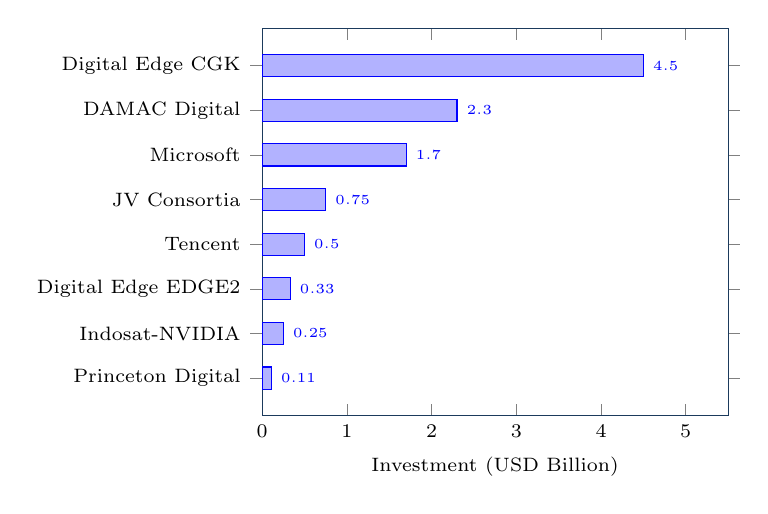
\begin{tikzpicture}
\begin{axis}[
    xbar,
    width=7.5cm,
    height=6.5cm,
    xlabel={Investment (USD Billion)},
    symbolic y coords={
        Princeton Digital,
        Indosat-NVIDIA,
        {Digital Edge EDGE2},
        Tencent,
        JV Consortia,
        Microsoft,
        DAMAC Digital,
        {Digital Edge CGK}
    },
    ytick=data,
    y tick label style={font=\scriptsize},
    x tick label style={font=\scriptsize},
    xlabel style={font=\scriptsize},
    nodes near coords,
    nodes near coords style={font=\tiny},
    every node near coord/.append style={anchor=west},
    xmin=0,
    xmax=5.5,
    bar width=8pt,
    enlarge y limits=0.12,
    fill=lightblue!80,
    draw=darkblue,
]
\addplot coordinates {
    (0.11,Princeton Digital)
    (0.25,Indosat-NVIDIA)
    (0.33,{Digital Edge EDGE2})
    (0.50,Tencent)
    (0.75,JV Consortia)
    (1.70,Microsoft)
    (2.30,DAMAC Digital)
    (4.50,{Digital Edge CGK})
};
\end{axis}
\end{tikzpicture}

\end{column}

\begin{column}{0.42\textwidth}
\begin{block}{Planned Capacity Additions}
\small
\begin{tabular}{lr}
\toprule
\textbf{Project} & \textbf{MW} \\
\midrule
DCI H2 Pertiwi   & 600 \\
Digital Edge CGK  & 500 \\
BDx Jatiluhur     & 500 \\
EdgeConneX JKT    & 200 \\
DAMAC Cikarang    & 144 \\
PDG (JC3+Batam)   & 118 \\
DayOne/INA Batam  & 72 \\
STT GDC Jakarta   & 72 \\
Telkom Cikarang   & 60 \\
NTT JKT2A+JKT3   & 57 \\
\bottomrule
\end{tabular}
\end{block}
\end{column}
\end{columns}

\end{frame}

% ============================================================
% SLIDE 4: Tax Incentives & Fiscal Cost
% ============================================================
\begin{frame}{Tax Incentives and Fiscal Cost}

\begin{columns}[T]
\begin{column}{0.48\textwidth}
\begin{block}{Tax Holiday (PMK 69/2024)}
\small
\begin{itemize}
    \item Data centers = \textbf{pioneer industry}
    \item \textbf{100\% CIT exemption} for 5--20 years\\ (investments $>$ IDR 500B / USD 33M)
    \item + 50\% reduction for 2 more years
    \item SEZs: \textbf{0\% VAT} on equipment imports ($\sim$11\% capex saving)
    \item 100\% foreign ownership allowed
\end{itemize}
\end{block}

\begin{alertblock}{OECD Pillar Two Impact}
\small
15\% global minimum tax $\Rightarrow$ Indonesia introducing domestic top-up tax (QDMTT) to retain revenue domestically. Recovers $\sim$USD 250M/yr.
\end{alertblock}
\end{column}

\begin{column}{0.48\textwidth}
\begin{block}{Estimated Fiscal Cost}
\small
\begin{tabular}{p{4.2cm}r}
\toprule
\textbf{Metric} & \textbf{Value} \\
\midrule
Total DC investment      & \$11.2B \\
Annual CIT foregone      & \$370M \\
10-yr cumulative cost    & \$3.7B \\
SEZ VAT foregone         & \$150M \\
\midrule
\textit{OECD recovery}   & \textit{--\$250M/yr} \\
\bottomrule
\end{tabular}
\end{block}

\begin{block}{But: Strong Leverage}
\small
\begin{itemize}
    \item Historical ratio: \textbf{18.5x}\\ (IDR 20T incentives $\to$ IDR 370T investment)
    \item 15--25K direct jobs
    \item Digital economy target: USD 130B
    \item Downstream VAT, property tax gains
\end{itemize}
\end{block}
\end{column}
\end{columns}

\end{frame}

\end{document}
